\chapter{AHTR Modeling and Optimization Methodology}
In this chapter, I describe the modeling and optimization methodology of
\gls{ROLLO} \gls{AHTR} optimization for non-conventional geometries and parameters.
To wholly explore the design space enabled by additive manufacturing, the 
optimization tool should enable placement of fuel, moderation, and coolant material 
in any possible location, within physical limits. 
Since exploration of non-conventional geometries and parameters has barely been
attempted (previous attempts described in Section \ref{sec:lit-review-reactor-arbitrary}), 
this dissertation attempts a first go at beginning to explore the large design space.  
The work done for this dissertation is only an intermediate step towards developing 
a truly arbitrary geometry expression. 

%In the subsequent sections, I will define the optimization problem, describe the 
%AHTR geometries . 
%Then, I will describe the software used to model them and the specific models. 

\section{Optimization Problem Definition}
In an effort towards optimizing reactor design for non-conventional geometries 
and parameters.
I chose to vary the following \gls{AHTR} parameters: 
\begin{itemize}
    \item \gls{TRISO} particle packing fraction distribution, 
    $\rho_{TRISO}(\vec{r})$
    \item Total fuel packing fraction
    \item \gls{FLiBe} coolant channel shape 
\end{itemize} 
The TRISO packing fraction distribution variation enables exploration of how 
heterogenous fuel distributions impact reactor performance;  
while the FliBe coolant channel shape variation enables exploration of how non-uniform 
channel shapes impact reactor performance. 

I selected three key \gls{AHTR} optimization objectives that address contrasting reactor 
core qualities. 
Table \ref{tab:objectives} describes each objective, how I quantified them, and the motivation.
\begin{table}[]
    \centering
    \onehalfspacing
    \caption{\acrfull{ROLLO} optimization problem objectives with their quantification 
    descriptions, and motivation.}
	\label{tab:objectives}
    \footnotesize
    \begin{tabular}{p{4cm}p{5cm}p{5cm}}
    \hline 
    \textbf{Objective}& \textbf{Quantification}& \textbf{Motivation} \\
    \hline
    Minimize fuel amount & Minimize total fuel packing fraction & Cost savings, Non-proliferation \\ 
    \hline
    Maximize heat transfer & Minimize maximum temperature & Enable system to perform at a higher power with minimized thermal stress \\
    \hline
    Minimize power peaking & Minimize power peaking factor normalized by fuel distribution & Efficient fuel utilization, longer core life, safety\\
    \hline
    \end{tabular}
\end{table}
I will be applying optimization process to the \gls{AHTR} plank and \gls{AHTR} one-third
assembly geometries.
The plank optimization acts as a preliminary study to inform the more complex \gls{AHTR} one-third
assembly optimization setup. 
In the next section, I will describe both geometries. 

\section{AHTR Geometry for Optimization Problem}
The optimization process is applied to both the \gls{AHTR} plank and \gls{AHTR} one-third
assembly geometries.
The geometries are slightly adapted from the \gls{AHTR} design in the \gls{FHR} benchmark,
outlined in Chapter \ref{chap:fhr-benchmark}.
The main changes occur in the fuel plank region (see Figure \ref{fig:ahtr-fuel-assembly}). 
In the \gls{FHR} benchmark, the TRISO particles are arranged in rectangular lattices within
two fuel stripes in the plank. 
For the optimization problem, I instead discretized each plank into ten cells with random 
TRISO packing and an individually controlled packing fraction. 
I also omit the graphite spacers. 

\subsection{AHTR Plank Geometry}
The \gls{AHTR} plank is a single graphite fuel plank model from the \gls{AHTR} design (Figure 
\ref{fig:ahtr-fuel-assembly}). 
I modified the fuel plank to be straightened with perpendicular sides, instead 
of slanted as in Figure \ref{fig:ahtr-fuel-plank}, for ease of modeling. 
The original \gls{AHTR} geometry will be used for the complex one-third assembly optimization 
setup. 
Figure \ref{fig:straightened_plank} illustrates the straightened fuel plank with 
fuel cell discretization with random \gls{TRISO} packing.
\begin{figure}[]
    \centering
    \includegraphics[width=0.85\linewidth]{straightened_plank.png}
    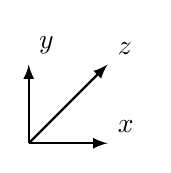
\begin{tikzpicture}
        \draw[ thick,-latex] (0,0) -- (1,0) node[anchor=south west] {$x$};
        \draw[ thick,-latex] (0,0) -- (0,1) node[anchor=south west] {$y$};
        \draw[ thick,-latex] (0,0) -- (1,1) node[anchor=south west] {$z$};
       \tkzText[above](-0.3,-0.7){}
       \end{tikzpicture} 
    \raggedright
    \resizebox{0.3\textwidth}{!}{
        \hspace{1cm}
        \fbox{\begin{tabular}{ll}
            \textcolor{fhrblue}{$\blacksquare$} & FLiBe \\
            \textcolor{fhrgrey}{$\blacksquare$} & Graphite (Fuel Plank)\\
            \textcolor{fhrred}{$\blacksquare$} & Graphite (Fuel Stripe) \\
            \textcolor{fhrblack}{$\blacksquare$} & TRISO particle 

            \end{tabular}}}
    \caption{Straightened \acrfull{AHTR} fuel plank with 10 fuel cells with random 
    TRISO packing. Original slanted fuel planks can be seen in Figures 
    \ref{fig:ahtr-fuel-assembly} and \ref{fig:ahtr-fuel-plank}.}
    \label{fig:straightened_plank}
\end{figure}
The plank has $27.1 \times 3.25 \times 1.85\ cm^3$ dimensions with reflective 
boundary conditions.

I use the same materials as in the \gls{FHR} benchmark (Chapter \ref{chap:fhr-benchmark}), 
except that I homogenized each \gls{TRISO} particle's four outer layers: 
porous carbon buffer, inner pyrolytic carbon, silicon carbide layer, and the 
outer pyrolytic carbon. 
The \gls{TRISO} particle dimensions remain the same.
Table \ref{tab:keff_triso} reports OpenMC's reported $k_{eff}$ for this original 
straightened \gls{AHTR} configuration with and without the outer layer \gls{TRISO} 
homogenization.
\begin{table}[]
    \centering
    \onehalfspacing
    \caption{Straightened \acrfull{AHTR} fuel plank $k_{eff}$ for case with 
    no \gls{TRISO} homogenization and case with homogenization of the four outer 
    layers. Both simulations were run on one BlueWaters XE Node.}
	\label{tab:keff_triso}
    \footnotesize
    \begin{tabular}{llc}
    \hline 
    \textbf{TRISO Homogenization}& \textbf{$k_{eff}$} & \textbf{Simulation time [s]}  \\
    \hline 
    None & $1.38548 \pm 0.00124$ & 233\\ 
    Four outer layers & $1.38625 \pm 0.00109$ & 168\\ 
    \hline
    \end{tabular}
\end{table}
The \gls{TRISO} particle outer four-layer homogenization resulted in a $30\%$ 
speed-up without compromising accuracy with $k_{eff}$ values within each 
other's uncertainty.

% fuel cell discretization for fuel distribution 
% coolant channel shape variation

\subsection{AHTR One-Third Assembly Geometry}
The \gls{AHTR} One-Third Assembly is one-diamond shape sector of the \gls{AHTR} assembly 
containing six fuel planks from the \gls{AHTR} design (Figure \ref{fig:ahtr-fuel-assembly}). 

\section{AHTR Model Workflow}

